%!TEX program=xelatex

\documentclass[11pt]{ctexart}  
\usepackage[top=2cm, bottom=2cm, left=2cm, right=2cm]{geometry}  
\usepackage{algorithm}  
\usepackage{algorithmicx}  
\usepackage{algpseudocode}  
\usepackage{amsmath}  
\usepackage{graphicx}
\usepackage{amsmath}
\usepackage{amssymb}
\usepackage{enumerate}
\usepackage{booktabs}

\floatname{algorithm}{算法}
\renewcommand{\algorithmicrequire}{\textbf{输入:}}  
\renewcommand{\algorithmicensure}{\textbf{输出:}} 

\title{密码学实验报告6}
\author{张天辰 17377321}

\makeatletter
\newenvironment{breakablealgorithm}
  {% \begin{breakablealgorithm}
   \begin{center}
     \refstepcounter{algorithm}% New algorithm
     \hrule height.8pt depth0pt \kern2pt% \@fs@pre for \@fs@ruled
     \renewcommand{\caption}[2][\relax]{% Make a new \caption
       {\raggedright\textbf{\ALG@name~\thealgorithm} ##2\par}%
       \ifx\relax##1\relax % #1 is \relax
         \addcontentsline{loa}{algorithm}{\protect\numberline{\thealgorithm}##2}%
       \else % #1 is not \relax
         \addcontentsline{loa}{algorithm}{\protect\numberline{\thealgorithm}##1}%
       \fi
       \kern2pt\hrule\kern2pt
     }
  }{% \end{breakablealgorithm}
     \kern2pt\hrule\relax% \@fs@post for \@fs@ruled
   \end{center}
  }
\makeatother

\begin{document}
\maketitle{}



\section{AES算法的查找表优化}
\subsection{查找表优化简介} % (fold)
AES的算法的耗时主要集中在有限域算术上。无论是字节代替、行移位还是轮密钥加,都只是简单的计算,唯有列混淆需要大量的计算时间。因为列混淆计算方式固定,所以可以用查找表的方式,用空间换取时间,大幅加快加解密速度。既然已经有了查找表的操作,就可以将字节代替和行移位也融合进去,进一步简化操作。在空间足够的场合,这种方式能极大地提高效率。
% subsection 查找表优化简介 (end)
\subsection{查找表生成原理} % (fold)
查找表方法基于如下事实(以下所有下标均在模4意义下):
\begin{enumerate}[(1)]
    \item 字节代替变换为:$$b_{i, j} = S[a_{i, j}]$$
    \item 行移位变换为:
    \begin{equation*}
    \begin{bmatrix}
    c_{0, j} \\ c_{1, j} \\ c_{2, j} \\ c_{3, j}
    \end{bmatrix}
    =
    \begin{bmatrix}
    b_{0, j} \\ b_{1, j+1} \\ b_{2, j+2} \\ b_{3, j+3}
    \end{bmatrix}
    \end{equation*}
    \item 列混淆变换为:
    \begin{equation*}
    \begin{bmatrix}
    d_{0, j} \\ d_{1, j} \\ d_{2, j} \\ d_{3, j}
    \end{bmatrix}
    =
    \begin{bmatrix}
        02 & 03 & 01 & 01 \\
        01 & 02 & 03 & 01 \\
        01 & 01 & 02 & 03 \\
        03 & 01 & 01 & 02
    \end{bmatrix}
    \begin{bmatrix}
    c_{0, j} \\ c_{1, j} \\ c_{2, j} \\ c_{3, j}
    \end{bmatrix}
    \end{equation*}
    \item 轮密钥加变换为:
    \begin{equation*}
    \begin{bmatrix}
    e_{0, j} \\ e_{1, j} \\ e_{2, j} \\ e_{3, j}
    \end{bmatrix}
    =
    \begin{bmatrix}
    d_{0, j} \\ d_{1, j} \\ d_{2, j} \\ d_{3, j}
    \end{bmatrix}
    \oplus
    \begin{bmatrix}
    k_{0, j} \\ k_{1, j} \\ k_{2, j} \\ k_{3, j}
    \end{bmatrix}
    \end{equation*}
\end{enumerate}
因此,可以将以上四种操作组合起来,即:
\begin{equation*}
    \begin{bmatrix}
    e_{0, j} \\ e_{1, j} \\ e_{2, j} \\ e_{3, j}
    \end{bmatrix}
    =
    \left(
    \begin{bmatrix}
    02 \\ 01 \\ 01 \\ 03
    \end{bmatrix}
    \cdot S[a_{0, j}] \right)
    \oplus
    \left(
    \begin{bmatrix}
    03 \\ 02 \\ 01 \\ 01
    \end{bmatrix}
    \cdot S[a_{1, j+1}] \right)
    \oplus
    \left(
    \begin{bmatrix}
    01 \\ 03 \\ 02 \\ 01
    \end{bmatrix}
    \cdot S[a_{2, j+2}] \right)
    \oplus
    \left(
    \begin{bmatrix}
    01 \\ 01 \\ 03 \\ 02
    \end{bmatrix}
    \cdot S[a_{3, j+3}] \right)
    \oplus
    \begin{bmatrix}
    k_{0, j} \\ k_{1, j} \\ k_{2, j} \\ k_{3, j}
    \end{bmatrix}
\end{equation*}
因此可以得到如下四个构造表的方式:
\begin{equation*}
     T_0[x] = 
     \left(
    \begin{bmatrix}
    02 \\ 01 \\ 01 \\ 03
    \end{bmatrix}
    \cdot S[x] \right) \quad
    T_1[x] = 
     \left(
    \begin{bmatrix}
    03 \\ 02 \\ 01 \\ 01
    \end{bmatrix}
    \cdot S[x] \right) \quad
    T_2[x] = 
     \left(
    \begin{bmatrix}
    01 \\ 03 \\ 02 \\ 01
    \end{bmatrix}
    \cdot S[x] \right) \quad
    T_3[x] = 
     \left(
    \begin{bmatrix}
    01 \\ 01 \\ 03 \\ 02
    \end{bmatrix}
    \cdot S[x] \right)
 \end{equation*} 
 于是,AES一轮加密可表示为:
 \begin{equation*}
    \begin{bmatrix}
    s'_{0, j} \\ s'_{1, j} \\ s'_{2, j} \\ s'_{3, j}
    \end{bmatrix}
    =
    T_0[s_{0, j}] \oplus T_1[s_{1, j+1}] \oplus T_2[s_{2, j+2}] \oplus T_3[s_{3, j+3}] \oplus 
    \begin{bmatrix}
    k_{0, j} \\ k_{1, j} \\ k_{2, j} \\ k_{3, j}
    \end{bmatrix}
 \end{equation*}
% subsection 查找表生成原理 (end)
\subsection{查找表AES加密的实现} % (fold)
以下算法展示了AES加密非首尾轮的查找表算法。
\begin{breakablealgorithm} 
\caption{查找表AES加密}
\begin{algorithmic}[1] %每行显示行号  
    \Function{encrypt}{}
    \For {$j \in [0, 3]$}
        \State $temp0 \gets t0[state[0][j]]$
        \State $temp1 \gets t1[state[1][(j+1)\%4]]$
        \State $temp2 \gets t2[state[2][(j+2)\%4]]$
        \State $temp3 \gets t3[state[3][(j+3)\%4]]$
        \For {$i \in [0, 3]$}
            \State $result[i][j] = temp0[i] \oplus temp1[i] \oplus temp2[i] \oplus temp3[i] \oplus key[i][j]$
        \EndFor
    \EndFor
    \EndFunction
\end{algorithmic}
\end{breakablealgorithm}
% subsection 查找表AES的实现 (end)
\subsection{AES查找表解密} % (fold)
解密查表与加密大同小异。主要的区别一方面是构造表的所用的矩阵不同,另一方面是对轮密钥加与逆向列混淆交换顺序的特殊处理。

四个解密表的构造为:
\begin{equation*}
     ReT_0[x] = 
     \left(
    \begin{bmatrix}
    0E \\ 09 \\ 0D \\ 0B
    \end{bmatrix}
    \cdot S^{-1}[x] \right) \quad
    ReT_1[x] = 
     \left(
    \begin{bmatrix}
    0B \\ 0E \\ 09 \\ 0D
    \end{bmatrix}
    \cdot S^{-1}[x] \right)
\end{equation*}
\begin{equation*}
    ReT_2[x] = 
     \left(
    \begin{bmatrix}
    0D \\ 0B \\ 0E \\ 09
    \end{bmatrix}
    \cdot S^{-1}[x] \right) \quad
    ReT_3[x] = 
     \left(
    \begin{bmatrix}
    09 \\ 0D \\ 0B \\ 0E
    \end{bmatrix}
    \cdot S^{-1}[x] \right)
 \end{equation*} 

在交换轮密钥加和逆向列混淆时,需要将轮密钥也做一次逆向列混淆。可用以下方式快速得到变换后的轮密钥:考虑到ReT表实质上是组合了逆S盒和逆向列混淆两种操作,因此为了只达到逆向列混淆的目的,可以先将轮密钥进行S盒变换,再查找ReT表,这样S盒和逆向S盒相互抵消,便只留下逆向列混淆操作。因此一轮解密可写为:
\begin{equation*}
    \begin{bmatrix}
    s'_{0, j} \\ s'_{1, j} \\ s'_{2, j} \\ s'_{3, j}
    \end{bmatrix}
    =
    ReT_0[s_{0, j}] \oplus ReT_1[s_{1, j-1}] \oplus ReT_2[s_{2, j-2}] \oplus ReT_3[s_{3, j-3}] \oplus ReT_0[k_{0, j}] \oplus ReT_1[k_{1, j}] \oplus ReT_2[k_{2, j}] \oplus ReT_3[k_{3, j}]
 \end{equation*}
% subsection aes查找表解密 (end)
\subsection{查找表AES解密的实现} % (fold)
以下算法展示了AES解密非首尾轮的查找表算法。
\begin{breakablealgorithm} 
\caption{查找表AES解密}
\begin{algorithmic}[1] %每行显示行号  
    \Function{encrypt}{}
    \For {$j \in [0, 3]$}
        \For {$i \in [0, 3]$}
            \State $temp \gets key[i][j]$
            \State $key[i][j] \gets S_BOX[temp//16][temp\%16]$
        \EndFor
    \EndFor
    \For {$j \in [0, 3]$}
        \State $temp0 \gets Ret0[state[0][j]]$
        \State $temp1 \gets Ret1[state[1][(j+1)\%4]]$
        \State $temp2 \gets Ret2[state[2][(j+2)\%4]]$
        \State $temp3 \gets Ret3[state[3][(j+3)\%4]]$
        \State $key\_temp0 \gets Ret0[key[0][j]]$
        \State $key\_temp1 \gets Ret1[key[1][j]]$
        \State $key\_temp2 \gets Ret2[key[2][j]]$
        \State $key\_temp3 \gets Ret3[key[3][j]]$
        \For {$i \in [0, 3]$}
            \State $result[i][j] = temp0[i] \oplus temp1[i] \oplus temp2[i] \oplus temp3[i] \oplus key\_temp0[i] \oplus key\_temp1[i] \oplus key\_temp2[i] \oplus key\_temp3[i]$
        \EndFor
    \EndFor
    \EndFunction
\end{algorithmic}
\end{breakablealgorithm}
\subsection{优化对比测试}
我选择了如下的测试方式:将优化前后的代码对同样大小的文件进行加密,并输出它们的代码执行时间,然后进行比较。测试得到的结果如下:
\begin{table}[h] 
    \centering 
    \caption{优化前后时间对比}
    \label{table_compare}
    \begin{tabular}{ccc}  
    \toprule[2pt]   
    文件大小 & 优化前加密时间 & 优化后加密时间\\  
    \midrule[1pt]   
    128 bit & 0.0182s & 0.00036s \\
    29 KB & 30.196s & 0.883s \\
    106KB & ? & 3.537s \\
    \bottomrule[2pt]  
    \end{tabular}
\end{table}
\begin{figure}[htbp]
\centering
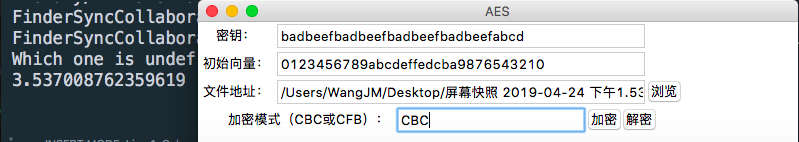
\includegraphics[height=1.42cm,width=7.99cm]{update.png}
\caption{优化后加密106KB文件}
\label{update}
\end{figure}

在文件大小达到100KB时,优化前的代码的加密速度过慢,整个程序无法响应,我只能将其关闭,这样的效率显然是没有实际意义的。总体来看,优化带来的速度加成是明显的。优化后的执行速度达到了30KB/s,效果令人满意。
\section{感想}

对于优化,我有几点心得:
\begin{enumerate}[(1)]
    \item 打表大概是理论上最快的解决方案,因为无论如何都是常数复杂度,代价就是占用空间。在目前的PC机上,这大可忽略不计。对于嵌入式系统,应该采取硬件编程方式,那和打表也无关了。
    \item 打表将速度提高了15倍,但最终的30倍速度提高有赖于我发现了deepcopy函数这个内鬼。我使用工具调试发现它占了好多时间,查资料才发现这个函数就是效率低下。果然优化之后时间又少了一半。
\end{enumerate}
此外,我正在尝试实现使用SIMD指令集优化AES算法,但是python语言无法采用这些指令,所以必然要在C++上重写AES,然后再应用指令集。Intel封装了这些指令,提供了一些接口函数。我希望自己能够完成这个任务。
\end{document}